%%%%%%%%%%%%%%%%%%%%%%%%%%%%%%%%%%%%%%%%%
% Programming/Coding Assignment
% LaTeX Template
%
% This template has been downloaded from:
% http://www.latextemplates.com
%
% Original author:
% Ted Pavlic (http://www.tedpavlic.com)
%
% Note:
% The \lipsum[#] commands throughout this template generate dummy text
% to fill the template out. These commands should all be removed when
% writing assignment content.
%
% This template uses a Perl script as an example snippet of code, most other
% languages are also usable. Configure them in the "CODE INCLUSION
% CONFIGURATION" section.
%
%%%%%%%%%%%%%%%%%%%%%%%%%%%%%%%%%%%%%%%%%

%----------------------------------------------------------------------------------------
%	PACKAGES AND OTHER DOCUMENT CONFIGURATIONS
%----------------------------------------------------------------------------------------

\documentclass{article}

\usepackage{fancyhdr} % Required for custom headers
\usepackage{lastpage} % Required to determine the last page for the footer
\usepackage{extramarks} % Required for headers and footers
\usepackage[usenames,dvipsnames]{color} % Required for custom colors
\usepackage{graphicx} % Required to insert images
\usepackage{caption}
\usepackage{subcaption}
\usepackage{listings} % Required for insertion of code
\usepackage{courier} % Required for the courier font
\usepackage{lipsum} % Used for inserting dummy 'Lorem ipsum' text into the template
\usepackage[T1]{fontenc}
\usepackage[utf8]{inputenc}
\usepackage{amsfonts}
\usepackage{amsthm,amsmath,amssymb}
\usepackage{cite}
\usepackage{hyperref}

\usepackage{color}
\newcommand{\todo}[1]{\textcolor{red}{TODO: #1}\PackageWarning{TODO:}{#1!}}

% Margins
\topmargin=-0.45in
\evensidemargin=0in
\oddsidemargin=0in
\textwidth=6.5in
\textheight=9.0in
\headsep=0.25in

\linespread{1.1} % Line spacing

% Set up the header and footer
\pagestyle{fancy}
\lhead{\hmwkTitle} % Top left header
%\chead{\hmwkClass\ (\hmwkClassInstructor\ \hmwkClassTime): \hmwkTitle} % Top center head
%\rhead{\firstxmark} % Top right header
\lfoot{\lastxmark} % Bottom left footer
\cfoot{} % Bottom center footer
\rfoot{Page\ \thepage\ of\ \protect\pageref{LastPage}} % Bottom right footer
\renewcommand\headrulewidth{0.4pt} % Size of the header rule
\renewcommand\footrulewidth{0.4pt} % Size of the footer rule

\setlength\parindent{0pt} % Removes all indentation from paragraphs

%----------------------------------------------------------------------------------------
%	CODE INCLUSION CONFIGURATION
%----------------------------------------------------------------------------------------

\definecolor{MyDarkGreen}{rgb}{0.0,0.4,0.0} % This is the color used for comments
\lstloadlanguages{Perl} % Load Perl syntax for listings, for a list of other languages supported see: ftp://ftp.tex.ac.uk/tex-archive/macros/latex/contrib/listings/listings.pdf
\lstset{language=Perl, % Use Perl in this example
        frame=single, % Single frame around code
        basicstyle=\small\ttfamily, % Use small true type font
        keywordstyle=[1]\color{Blue}\bf, % Perl functions bold and blue
        keywordstyle=[2]\color{Purple}, % Perl function arguments purple
        keywordstyle=[3]\color{Blue}\underbar, % Custom functions underlined and blue
        identifierstyle=, % Nothing special about identifiers
        commentstyle=\usefont{T1}{pcr}{m}{sl}\color{MyDarkGreen}\small, % Comments small dark green courier font
        stringstyle=\color{Purple}, % Strings are purple
        showstringspaces=false, % Don't put marks in string spaces
        tabsize=5, % 5 spaces per tab
        %
        % Put standard Perl functions not included in the default language here
        morekeywords={rand},
        %
        % Put Perl function parameters here
        morekeywords=[2]{on, off, interp},
        %
        % Put user defined functions here
        morekeywords=[3]{test},
       	%
        morecomment=[l][\color{Blue}]{...}, % Line continuation (...) like blue comment
        numbers=left, % Line numbers on left
        firstnumber=1, % Line numbers start with line 1
        numberstyle=\tiny\color{Blue}, % Line numbers are blue and small
        stepnumber=5 % Line numbers go in steps of 5
}

% Creates a new command to include a perl script, the first parameter is the filename of the script (without .pl), the second parameter is the caption
\newcommand{\perlscript}[2]{
\begin{itemize}
\item[]\lstinputlisting[caption=#2,label=#1]{#1.pl}
\end{itemize}
}

%----------------------------------------------------------------------------------------
%	DOCUMENT STRUCTURE COMMANDS
%	Skip this unless you know what you're doing
%----------------------------------------------------------------------------------------

% Header and footer for when a page split occurs within a problem environment
\newcommand{\enterProblemHeader}[1]{
\nobreak\extramarks{#1}{#1 continued on next page\ldots}\nobreak
\nobreak\extramarks{#1 (continued)}{#1 continued on next page\ldots}\nobreak
}

% Header and footer for when a page split occurs between problem environments
\newcommand{\exitProblemHeader}[1]{
\nobreak\extramarks{#1 (continued)}{#1 continued on next page\ldots}\nobreak
\nobreak\extramarks{#1}{}\nobreak
}

\setcounter{secnumdepth}{0} % Removes default section numbers
\newcounter{homeworkProblemCounter} % Creates a counter to keep track of the number of problems

\newcommand{\homeworkProblemName}{}
\newenvironment{homeworkProblem}[1][Problem \arabic{homeworkProblemCounter}]{ % Makes a new environment called homeworkProblem which takes 1 argument (custom name) but the default is "Problem #"
\stepcounter{homeworkProblemCounter} % Increase counter for number of problems
\renewcommand{\homeworkProblemName}{#1} % Assign \homeworkProblemName the name of the problem
\section{\homeworkProblemName} % Make a section in the document with the custom problem count
\enterProblemHeader{\homeworkProblemName} % Header and footer within the environment
}{
\exitProblemHeader{\homeworkProblemName} % Header and footer after the environment
}

\newcommand{\problemAnswer}[1]{ % Defines the problem answer command with the content as the only argument
\noindent\framebox[\columnwidth][c]{\begin{minipage}{0.98\columnwidth}#1\end{minipage}} % Makes the box around the problem answer and puts the content inside
}

\newcommand{\homeworkSectionName}{}
\newenvironment{homeworkSection}[1]{ % New environment for sections within homework problems, takes 1 argument - the name of the section
\renewcommand{\homeworkSectionName}{#1} % Assign \homeworkSectionName to the name of the section from the environment argument
\subsection{\homeworkSectionName} % Make a subsection with the custom name of the subsection
\enterProblemHeader{\homeworkProblemName\ [\homeworkSectionName]} % Header and footer within the environment
}{
\enterProblemHeader{\homeworkProblemName} % Header and footer after the environment
}

%----------------------------------------------------------------------------------------
%	NAME AND CLASS SECTION
%----------------------------------------------------------------------------------------

\newcommand{\hmwkTitle}{Image classification using Vietoris-Rips complex} % Assignment title
\newcommand{\hmwkDueDate}{Friday,\ May\ 13,\ 2016} % Due date
\newcommand{\hmwkClass}{Computational topology} % Course/class
\newcommand{\hmwkClassTime}{} % Class/lecture time
\newcommand{\hmwkClassInstructor}{Neža Mramor Kosta, Gregor Jerše} % Teacher/lecturer
\newcommand{\hmwkAuthorName}{Andrej Dolenc, Peter Us, Rok Ivanšek} % Your name

% Comands for theorems, definitions, other
\newtheorem{definition}{Definition}
\newtheorem{claim}{Claim}
%----------------------------------------------------------------------------------------
%	TITLE PAGE
%----------------------------------------------------------------------------------------

\title{
\vspace{2in}
\textmd{\textbf{\hmwkClass:\ \hmwkTitle}}\\
% \normalsize\vspace{0.1in}\small{Due\ on\ \hmwkDueDate}\\
\normalsize\vspace{0.1in}\small{\today}\\
\vspace{0.1in}\large{\textit{\hmwkClassInstructor\ \hmwkClassTime}}
\vspace{3in}
}

\author{\textbf{\hmwkAuthorName}}
\date{} % Insert date here if you want it to appear below your name

%----------------------------------------------------------------------------------------

\begin{document}

\maketitle

%----------------------------------------------------------------------------------------
%	TABLE OF CONTENTS
%----------------------------------------------------------------------------------------

%\setcounter{tocdepth}{1} % Uncomment this line if you don't want subsections listed in the ToC

\newpage
\tableofcontents
\newpage

%----------------------------------------------------------------------------------------
%	Project description
%----------------------------------------------------------------------------------------

\begin{homeworkProblem}[Project description]
As the title implies, the idea behind the project is to use the Vietoris-Rips (in future abreviated VR-cx) complex for image classification. We took pictures of three generic objects and preprocessed them so we obtained vector representations of pictures. The vector representations of images can then be looked upon as points in some $n$-dimensional space $\mathbb{R}^{n}$. Over this points we build the VR-cx for two different parameters. We use the complexes to build a classification model for the images and classify them. We also perform several interesting tests on the generated VR-cx.
\end{homeworkProblem}

%----------------------------------------------------------------------------------------
%	Obtaining and preprocessing data
%----------------------------------------------------------------------------------------

% To have just one problem per page, simply put a \clearpage after each problem

\begin{homeworkProblem}[Obtaining and preprocessing data]
%Listing \ref{homework_example} shows a Perl script.

\begin{figure}[t!]
    \centering
    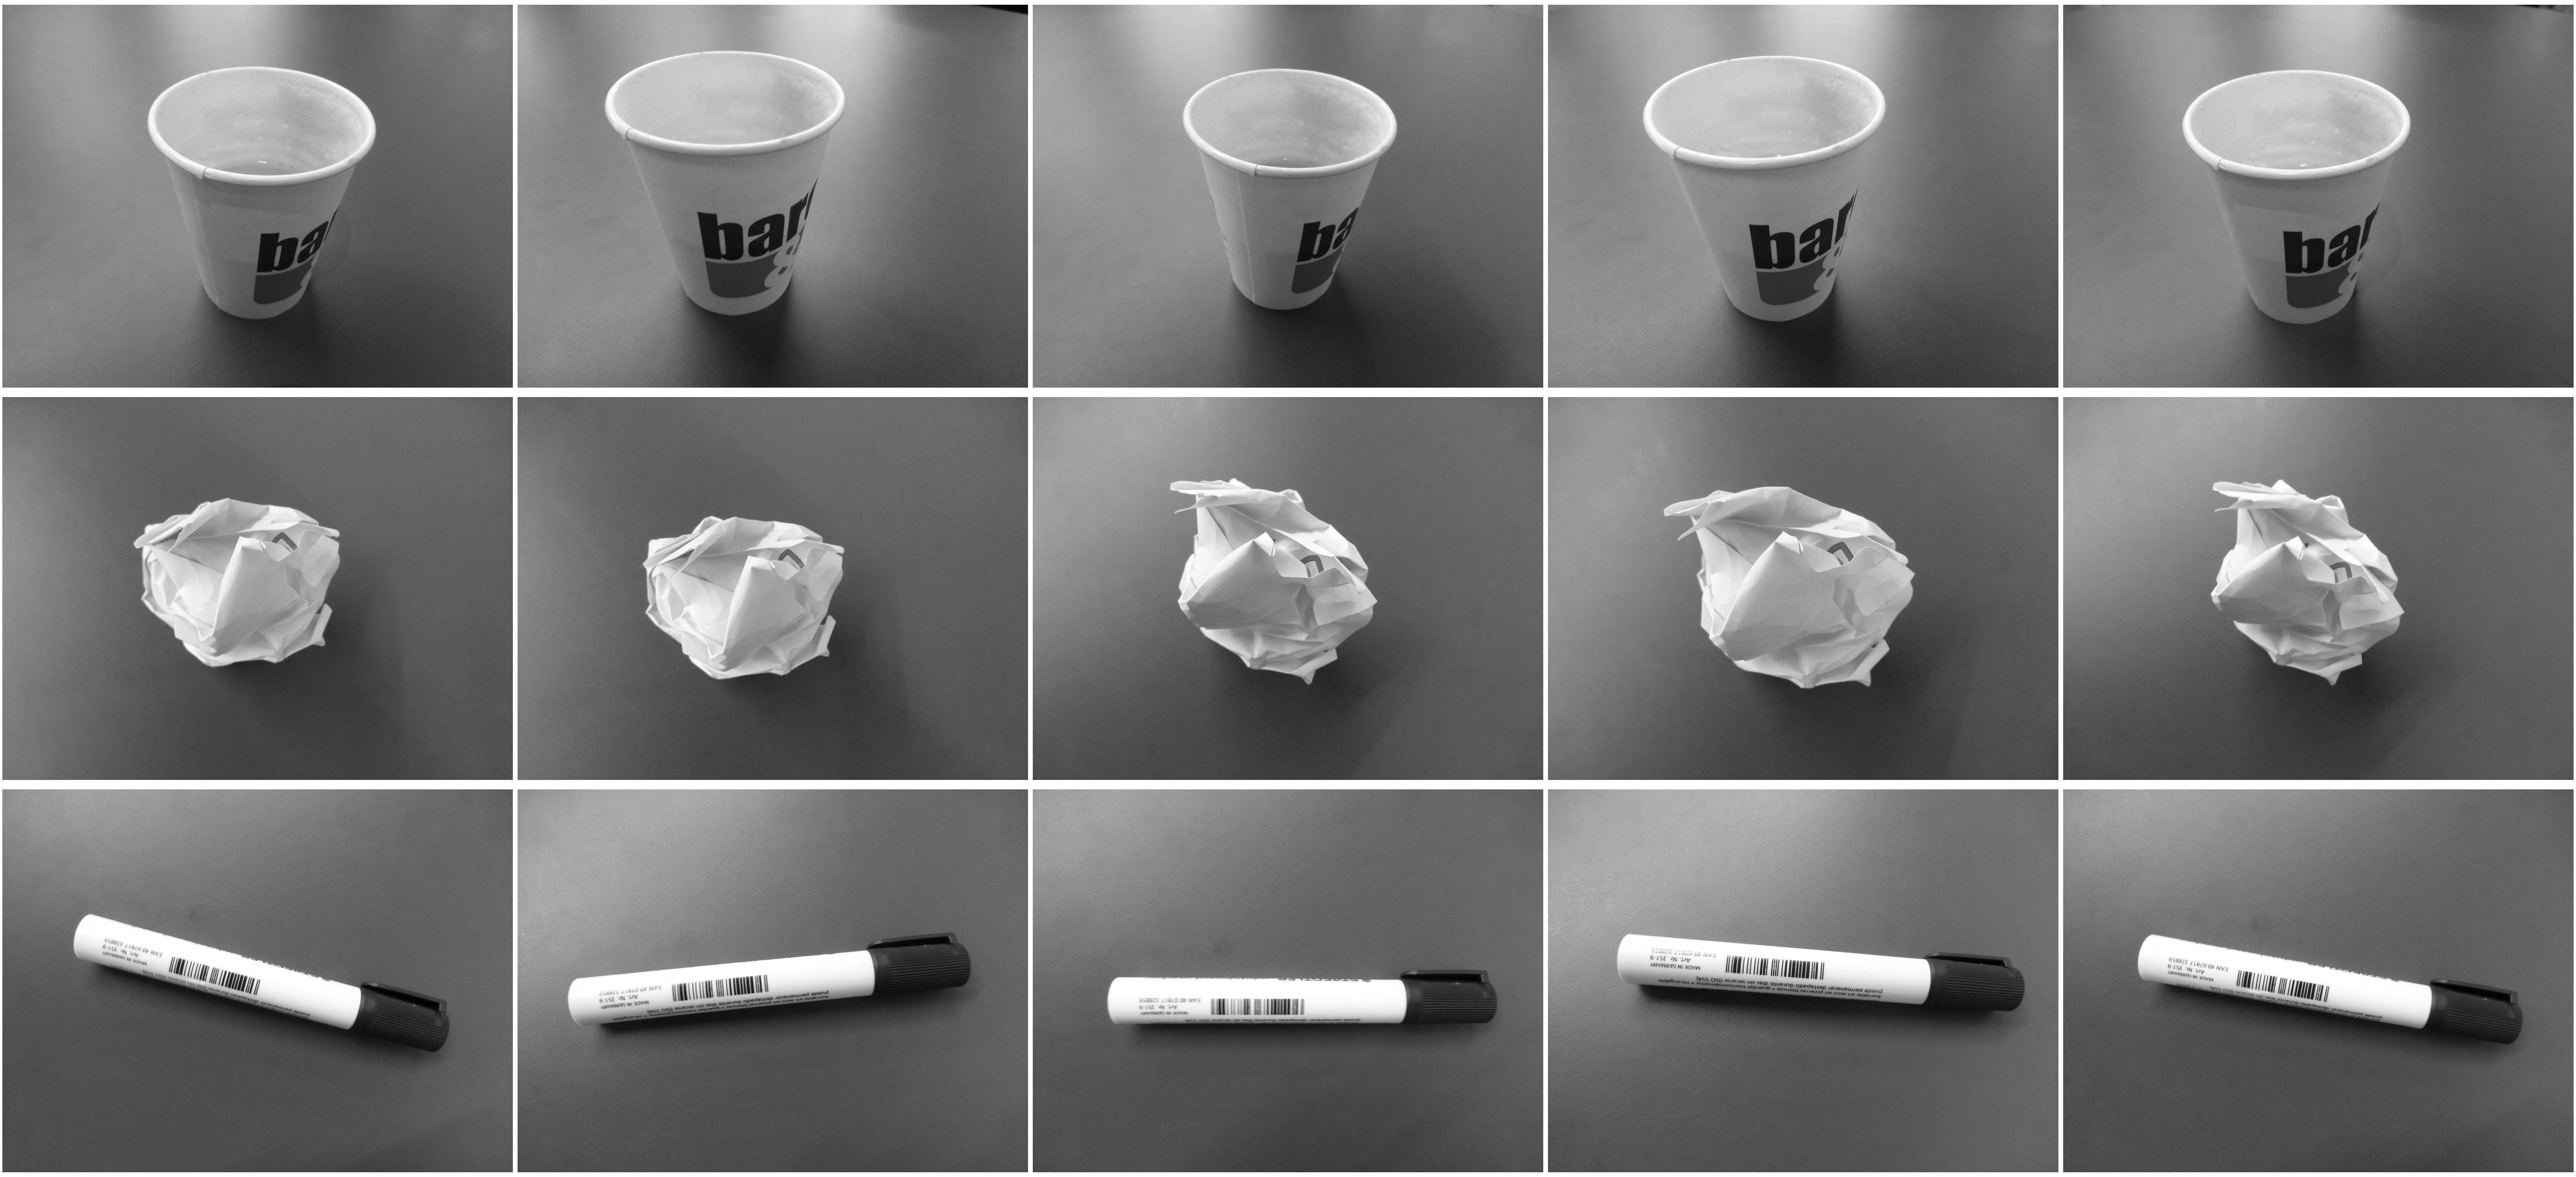
\includegraphics[height=7.5cm]{img/dataset}
    \caption{Sample images from used dataset.}
    \label{fig:data}
\end{figure}

\begin{figure}[t!]
    \centering
    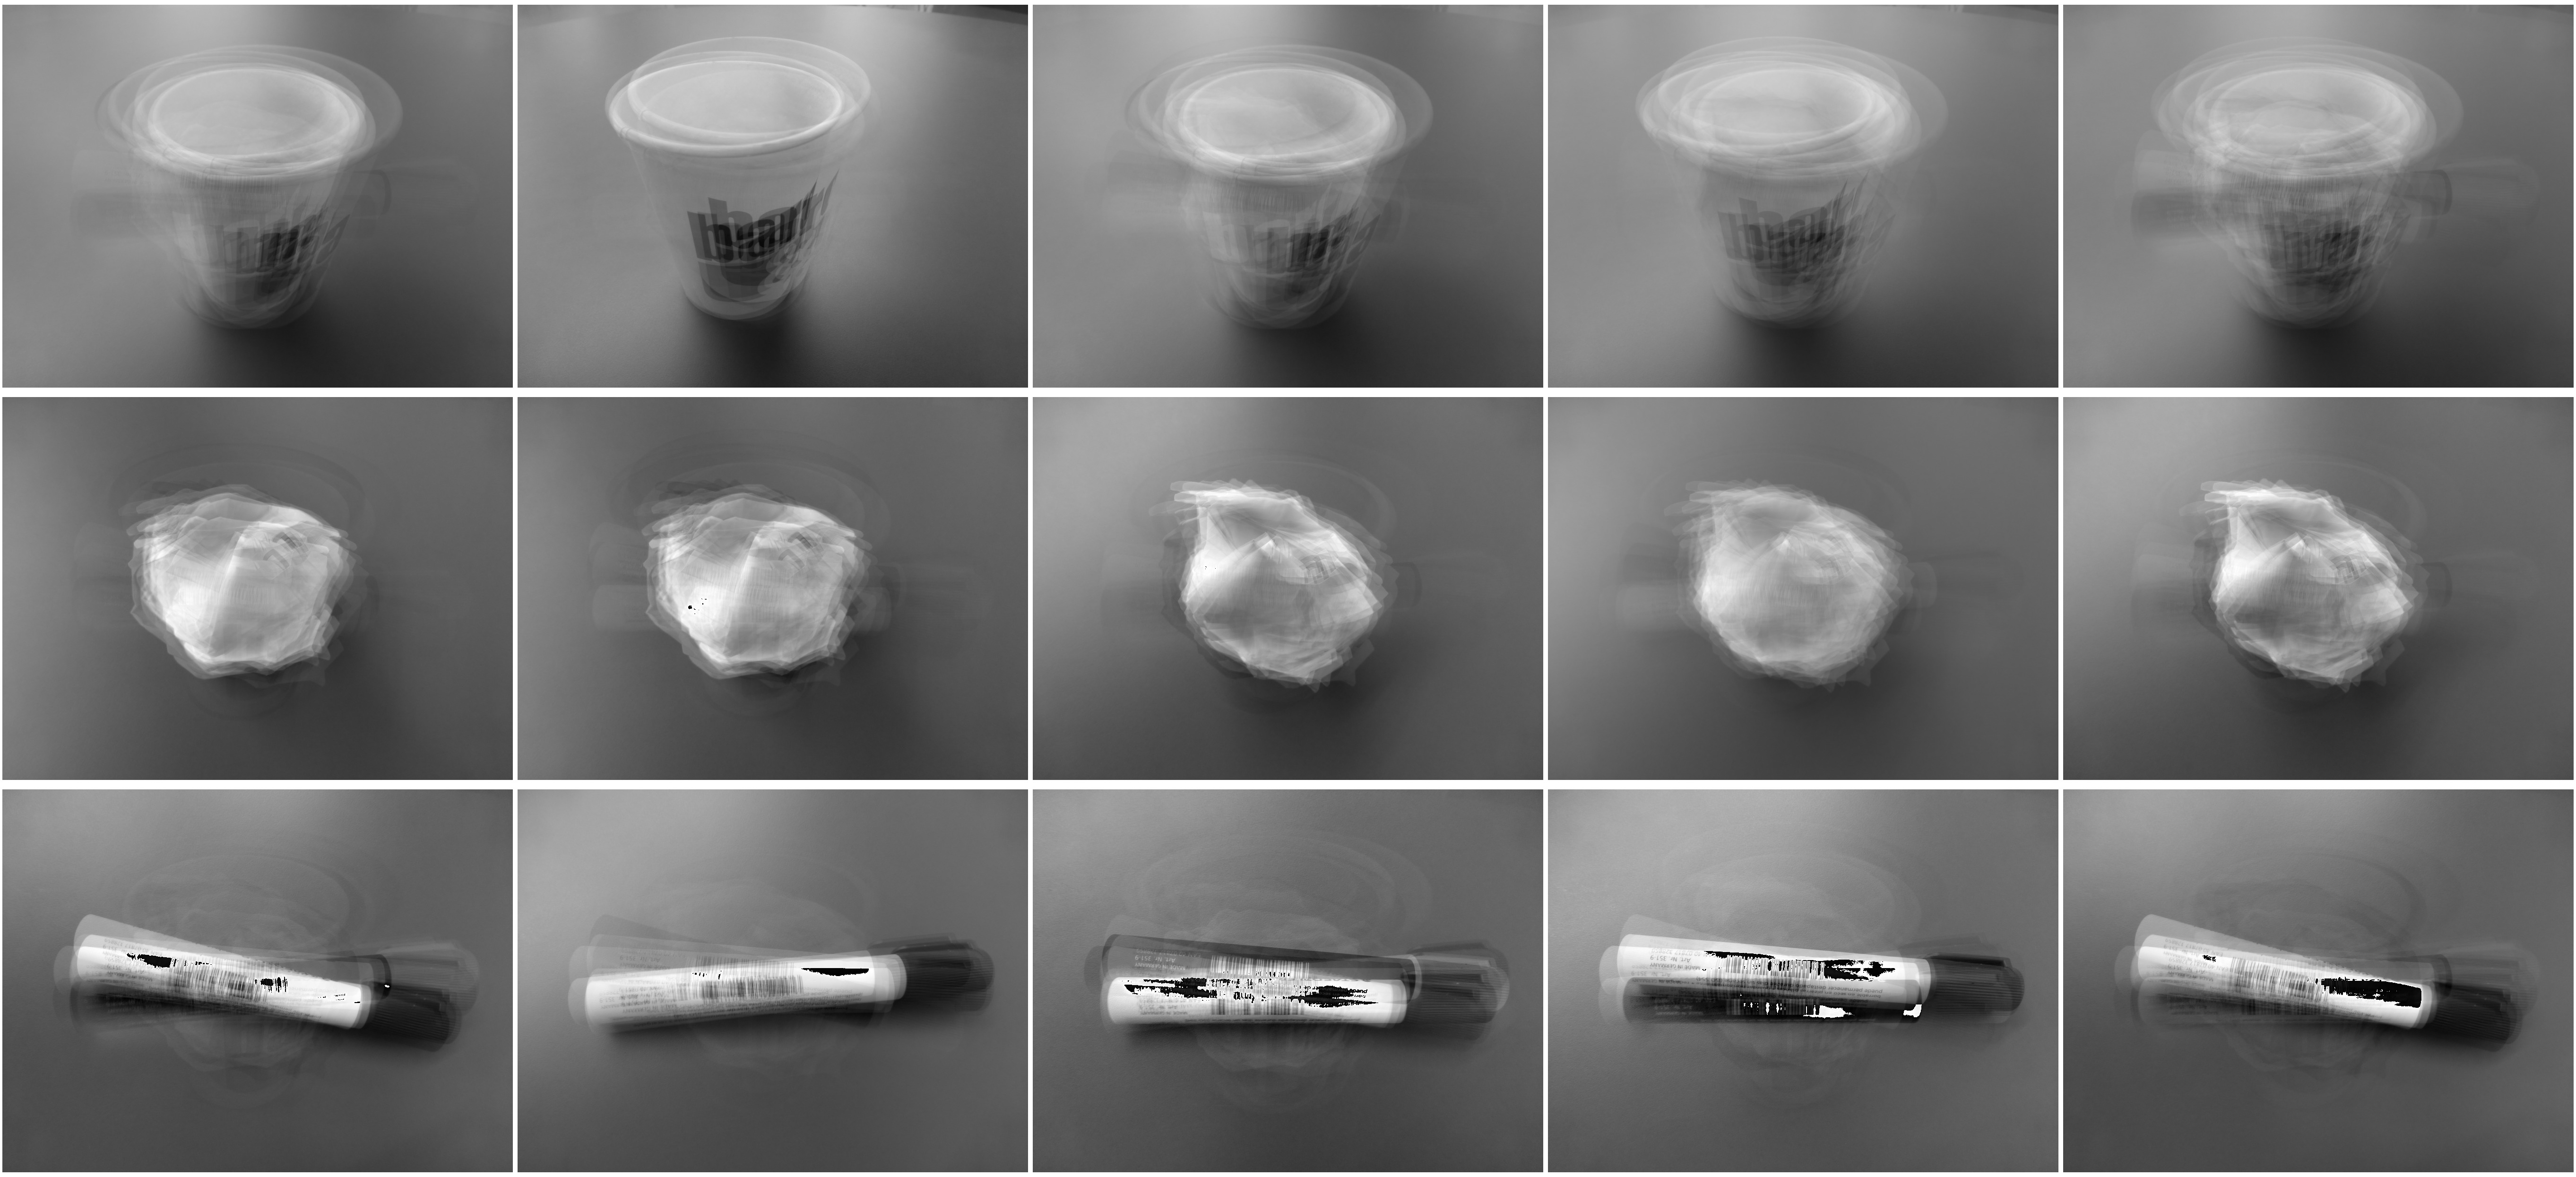
\includegraphics[height=7.5cm]{img/inverse_dataset}
    \caption{Images from figure \ref{fig:data} after applying preprocessing and inverse preprocessing steps to them. \todo{No reference anywhere in the text}}
    \label{fig:inv}
\end{figure}

For our dataset we used grayscale photographs of 3 different objects: a paper cup, crumpled up paper and a pen. Each of the objects was photographed 10 times from slightly different angles and under different illumination. The sizes of the images were $1080$ pixels in width and $810$ pixels in height. A selection of these photographs can be seen in figure \ref{fig:data}.

  We can think of images as matrices of size $(n \times m)$ where each entry represents the intensity of the corresponding pixel (meaning in our case we had $30$ matrices of size $1080 \times 810$). With images in grayscale color space, each of the values is an integer between $0$ (black) and $255$ (white). In order to prepare the dataset for evaluation with our classification model, we flattened image's matrix into one long vector of size $n m$ (first row of the matrix being first $n$ elements, second row the next $n$ and so on $m$ times). We then stacked all individual vectors vertically to form a large matrix with $30$ rows, one for each individual image, and $n m$ columns, one for each individual pixel.

  Because we wanted to help our model as much as possible via preprocessing, we scaled/transformed the values of each pixel either using a standard scaler, or by subtracting mean and scaling values to the $[-1, 1]$ interval. The main motivation behind this was to remove varying illumination from our dataset.

With this however we are still left with a matrix of very high dimensions, so in order to reduce processing time, decrease redundancy and amount of noise, we apply principal component analysis to it. With this we can to reduce the number of columns from $n \times m$ to but a few which makes the dataset much more manageable.
\end{homeworkProblem}

%----------------------------------------------------------------------------------------
%	The classification model
%----------------------------------------------------------------------------------------

\begin{homeworkProblem}[The classification model] \label{prob:model}

\begin{definition}[Vietoris-Rips complex]
\label{defa}
Let $X$ be a set of $m$-dimensional points $X \in \mathbb{R}^{m}$ and let $d$ be a metric. Pick a parameter $r > 0$. Construct a simplicial complex as follows:
\begin{itemize}
	\item Add a $0$-simplex for each point in $X$.
	\item For $x_{1}, x_{2} \in X$ add a $1$-simplex between $x_{1}, x_{2}$ if $d(x_{1}, x_{2}) \leq r$.
	\item For $x_{1}, x_{2}, x_{3} \in X$ add a $2$-simplex with vertices $x_{1}, x_{2}, x_{3}$ if $d(x_{1}, x_{2}), d(x_{1}, x_{3}), d(x_{2}, x_{3}) \leq r$.
	\item ...
	\item For $x_{1}, x_{2}, ... , x_{m} \in X$, add a $(m-1)$-simplex with vertices $x_{1}, x_{2}, ..., x_{m}$ if $d(x_{i}, x_{j}) \leq r$ for $0 \leq i,j \leq m$; that is, if all the points are within a distance of $r$ from each other.
\end{itemize}
The simplicial complex is called the Vietoris-Rips complex and is denoted $VR_{r}(X)$.
\end{definition}

\begin{definition}
We say that disjoint subsets $A_{1}...A_{k}$ of vertices $V$ in graph $G(V,E)$ are $k$ connected components of the graph $G$ if the following is true:
\begin{enumerate}
	\item The vertices inside $A_{i}$ are connected i.e. there exists a path between arbitrary two vertices $a, b \in A_{i}$, for every $i \in 1...k$.
	\item The sets of vertices $A_{1},...,A_{k}$ are disconnected i.e. there isn't an edges $e(a, b)$ between a pair of two points $(a,b)$ such that $a \in A_{i}, b \in A_{j}, i \neq j$.
\end{enumerate}
\end{definition}

Given the input of $n$ $m$-dimensional points $X \in \mathbb{R}^{m}$ and a metric $d$ (in our case the eulidian distance) we build a VR-cx for parameter $r = r_{2}$, where $r_{2}$ is the biggest $r$ such that the VR-cx has three connected components. We find the parameter $r_{2}$ using a binary search on a set of all possible values of $r$. We then perform the classification, simply by saying that all the objects in some connected component belong to the same class. Seeing as we have three connected components in our VR-cx we will get three distinct classes.\\

It does not take much thought to see, that our classification model will produce the exact same results if we  only use simplices of dimension $1$, as it would, if we use all the simplices up to dimension $h$, where $h$ is an arbitrary number in the range $h \in 1...m$. This follows from Definition~\ref{defa}.

\begin{homeworkSection}{Relation to single linkage clustering algorithm}

Our intuition tells us, that the model we build using the VR-cx to classify the images, produces the same results as the well known single linkage clustering algorithm. In this section we aim to prove or at least give a strong intuition that this is indeed the case.

Both algorithms take a set $X$ of $n$ samples with $m$ features as input. We can think of a sample $x$ in the set $X$ as a point in the $m$-dimensional space $x \in \mathbb{R}^{m}$. The algortihms then constructs a graph with points $X$ as the vertices ($V$) and edges $E$. The $k$ connected components in the constructed graph corespond to the classes of samples.

\begin{paragraph}{Single linkage algorithm.}
The algorithm starts with $n$ connected components (no edges in the graph). n each step the algorithm chooses the two connected components that are closest to each according to some distance metric $d$ (in our case the euclidean distance) and joins them into one by adding an edge between their closest two vertices.

\begin{definition}
The distance $D$ between two connected components $A$ and $B$ is defined as the distance of the pair of vertices (one from $A$ and one from $B$) that are closest to each other. More formally
$$D(A, B) =  \min_{a \in A, b \in B} d(a,b).$$
\end{definition}

The algorithm stops when there are only $k$ connected components left.

\end{paragraph}

\begin{paragraph}{Vietoris-Rips classification algorithm.}
The algorithm builds a ($1$-dimensional) Vietoris-Rips complex $V_{r}(X)$ with parameter $r$. We choose the biggest $r$ such that the Vietoris-Rips complex $V_{r}(X)$ has $k$ connected components.
\end{paragraph}
\\
\\
To prove that the two algorithms indeed produce the same connected components we will first prove the next claim.

\begin{claim}\label{claima}
Let $G_{sl}(V, E_{sl})$ be a graph produced by the single linkage algorithm for finding $k$ clusters and let $d_{max}$ denote the distance between vertices in graph $G_{sl}$ that were connected in the last iteration of the algorithm. Graph $G_{sl}$ has connected components $A_{1}...A_{k}$. The graph $G_{vr}(V, E_{vr})$ induced by the Vietoris-Rips complex $VR_{d_{max}}(V)$ has the same connected components $A_{1}...A_{k}$.
\end{claim}

\begin{proof}
We prove the Claim~\ref{claima} by induction on the steps in the single linkage algorithm. We start with a set of vertices $V$. Let $j$ denote the step (iteration) of the algorithm, $e_{j}$ the edge added in $j$-th step and $d_{j}$ its length. We claim that at each $j$ the graph $G_{sl}^{j}$ constructed by the algorithm up to that point, has the exact same conected components as $G_{vr}^{j}$, that is the graph induced by the Vietoris-Rips complex $VR_{d_{j}}(V)$.

\begin{paragraph}{Base case.}For $j=0$ this is obvious, since this is the initial state of the algorithm. Both graphs $G_{sl}^{0}$ and $G_{vr}^{0}$ consist only of vertices $V$. For $j=1$ the algorithm adds the smallest edge $e_{1}$ out of all possible candidates and builds a graph $G_{sl}^{1}$. Edge $e_{1}$ has length $d_{1}$. It is obvious that $VR_{d_{1}}(V)$ will induce a graph $G_{vr}^{1}$ that will also only contain edge $e_{1}$, since no other pairwise distance between vertices $V$ is smaller.
\end{paragraph}

\begin{paragraph}{Induction step.}
Here we show that if for some $j$ our claim holds, it will also hold after another iteration of the algorithm i.e. for $j+1$. In $(j+1)$-th iteration, the algortihm finds the edge $e_{j+1}$ with length $d_{j+1}$ and adds it to the graph. By the definition of the algortihm $e_{j+1}$ is the smallest such edge that connects (joins) two seperate connected components. This means that every other edge $e'$ with length $d' < d_{j+1}$ would not join connected components, but would instead just connect two vertices, that are both allready in the same connected component. From the definition of the Vietoris-Rips complex we can see that in the graph $G_{vr}^{j+1}$ there will only be one new edge that will join two seperate connected components, and that will be exactly edge $e_{j+1}$. All the other extra edges that will be added in $G_{vr}^{j+1}$, but do not appear in  $G_{sl}^{j+1}$ have length less than $d_{j+1}$ and will therefore only connect vertices inside of allready existing connected components of the graph $G_{vr}^{j}$. Since by our induction hypothesis graphs $G_{sl}^{j}$ and $G_{vr}^{j}$ had the same connected components and we joined two of the same connected components in both graphs, this means that the graphs $G_{sl}^{j+1}$ and $G_{vr}^{j+1}$ also have the same connected components.
\end{paragraph}\\
\\
We have proven that the graph $G_{sl}^{j}$ constructed in $j$-th iteration of the single linkage algorithm indeed contains the same connected commponents as the graph $G_{vr}^{j}$ induced by $VR_{d_{j}}(V)$ for an arbitrary $j$. This also prooves Claim~\ref{claima}.
\end{proof}

Using Claim~\ref{claima} we see that the connected components in $G_{vr}$ and $G_{sl}$ are indeed the same. We need to take into account that the Vietrois-Rips algorithm takes the biggest such $r$, so that the graph has $k$ connected components, so $r > d_{max}$. But we can quickly see that the extra edges in the graph induced by $V_{r}(V_{sl})$ will not change the connected components. After all we allready have $k$ connected components in $G_{vr}$. To join any two together would mean a violation of a fundemental rule of the algorithm.

\end{homeworkSection}

\begin{homeworkSection}{Computational complexity}

  Let us now consider the computational complexity of our model. Since we are only interested in Vietoris-Rips complexes $VR_r$ with simplices of dimension $1$, the simplest approach to construct such complex requires us to check the distance between every pair of vertices $(x_1, x_2) \in X \times X$, adding such pair to the final complex if the distance $d(x_1, x_2) \le r$. In worst case the algorithm would have to return all distinct pairs of vertices, meaning construction of $VR_r(X)$ requires $O(n^2)$ time and consumes $O(n^2)$ space, where $n$ is the number of vertices in $X$.

  The problem is that we don't know the appropriate value for the parameter $r$. Recall that we are interested in finding biggest $r$, such that the Vietoris-Rips complex $VR_{r}$ has as many connected components as there are distinct classes of images. Let $r_{max}$ denote the largest distance between two vertices from $X$. Note that $r$ we are looking for will always be bounded on the interval $[0, r_{max}]$, and it will furthermore be exactly one of the distances between some pair of vertices. Thus we only have $n^2$ different possible values of $r$ to check, and if we sort them by size and use binary search to find the right one, we can do it in $O(n^2 \log n^2) = O(n^2 \log n)$ time and $O(n^2)$ space. To count the number of connected components obtained with every different $VR$ complexes, we can use a \texttt{union-find} algorithm, which at worst adds $O(n^2)$ time to each run.

  With this the final time complexity of our approach is $O(n^2 \log n^2 + (n^2 + n^2)\log n^2) = O(n^2 \log n)$ using $O(n^2)$ space. Contrast this with the computational complexity of single-linkage clustering, which with a clever implementation can in optimal case produce solution in $O(n^2)$ time and $O(n)$ space~\cite{gower1969minimum}.

\end{homeworkSection}


%\begin{center}
%\includegraphics[width=0.75\columnwidth]{example_figure} % Example image
%\end{center}


\end{homeworkProblem}

\begin{homeworkProblem}[Results]

\begin{homeworkSection}{Cup, paper, pen image set}

\begin{paragraph}{Effect of preprocessing}
We were interested in observing the effect of the preprocessing methods on the samples of our dataset. For this purpose we visualized the data-points using multidimensional scaling technique (MDS)~\cite{borg2005modern}. MDS is a means of visualizing the level of similarity of individual cases from $N$-dimensional space, to a lower, $M$ dimensional space (in our case: $M=2$), while preserving between-object distances as good as possible. Therefore MDS plots are well suited for giving intuition of how separable data samples of different classes are. The obtained plots are shown in figure~\ref{fig:mds_preprocessing}. We notice that in both cases the points can be clearly separated into three clusters. We can also observe that points within clusters seem to lie closer together in the preprocessed plot than in the non preprocessed one. It should be mentioned that the position of points in a MDS plot is randomized, and that only distances between points should be observed. Therefore the reader should not confuse the different positions of each of the clusters in the plots as an effect of the preprocessing, since the reason for it is merely a property of the MDS method.

\begin{figure}[t]
    \centering
    \begin{subfigure}[t]{0.4\textwidth}
        \centering
        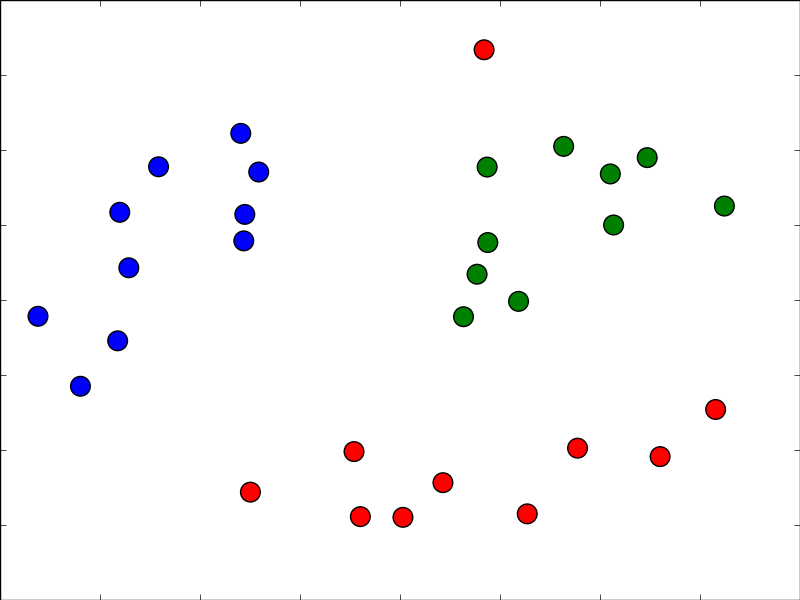
\includegraphics[height=3.5cm]{img/mds_no_preprocessing}
    \end{subfigure}
   ~
    \begin{subfigure}[t]{0.4\textwidth}
        \centering
        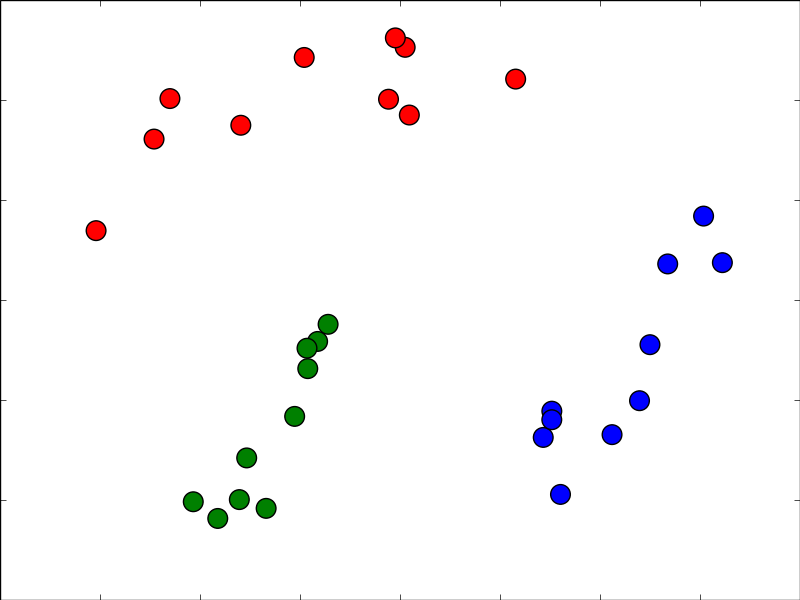
\includegraphics[height=3.5cm]{img/mds_preprocessing}
        \end{subfigure}
  \caption{MDS plots visualizing cup (blue), paper (red), and pen (green) samples from the dataset. Left figure is the original dataset. Right figure shows the scaled and PCA transformed dataset. Euclidean distance metric was used.}
  \label{fig:mds_preprocessing}
\end{figure}

\end{paragraph}

\begin{paragraph}{Image classification.}  In this section we present the results of Vietoris-Rips classification algorithm described in section~\ref{prob:model}. \todo{Why is this reference not shown?}

\begin{figure}[h]
    \centering
    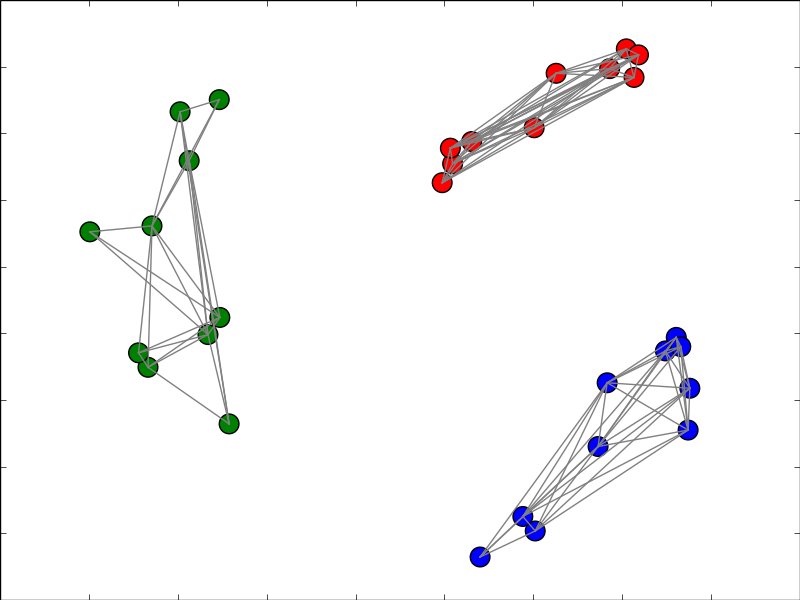
\includegraphics[height=5cm]{img/vr_cx}
    \caption{Visualisation of the VR-cx on the cup, paper, and pen dataset.}
    \label{fig:vr_cx}
\end{figure}


Initially we tested if the model is able to distinguish the images of cup, paper and pen. The images were preprocessed with scaling and a PCA transformation. The VR-cx obtained is shown in fig~\ref{fig:vr_cx}. The model had no problems distinguishing between the three classes of images. Each one of the three connected components obtained was belonging to one of the three classes of images. This is not surprising as the three classes of points are clearly separable.
\end{paragraph}

\begin{figure}[h]
    \centering
    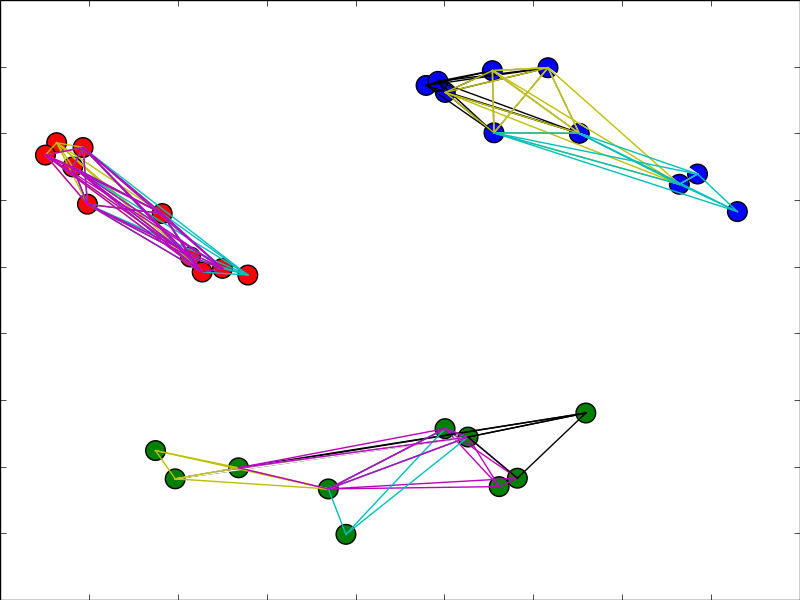
\includegraphics[height=5cm]{img/vr_princ}
    \caption{Visualisation of the principal simplicies obtained by VR-cx on the cup, paper, and pen dataset.}
    \label{fig:vr_princ}
\end{figure}

\begin{figure}[h]
    \centering
    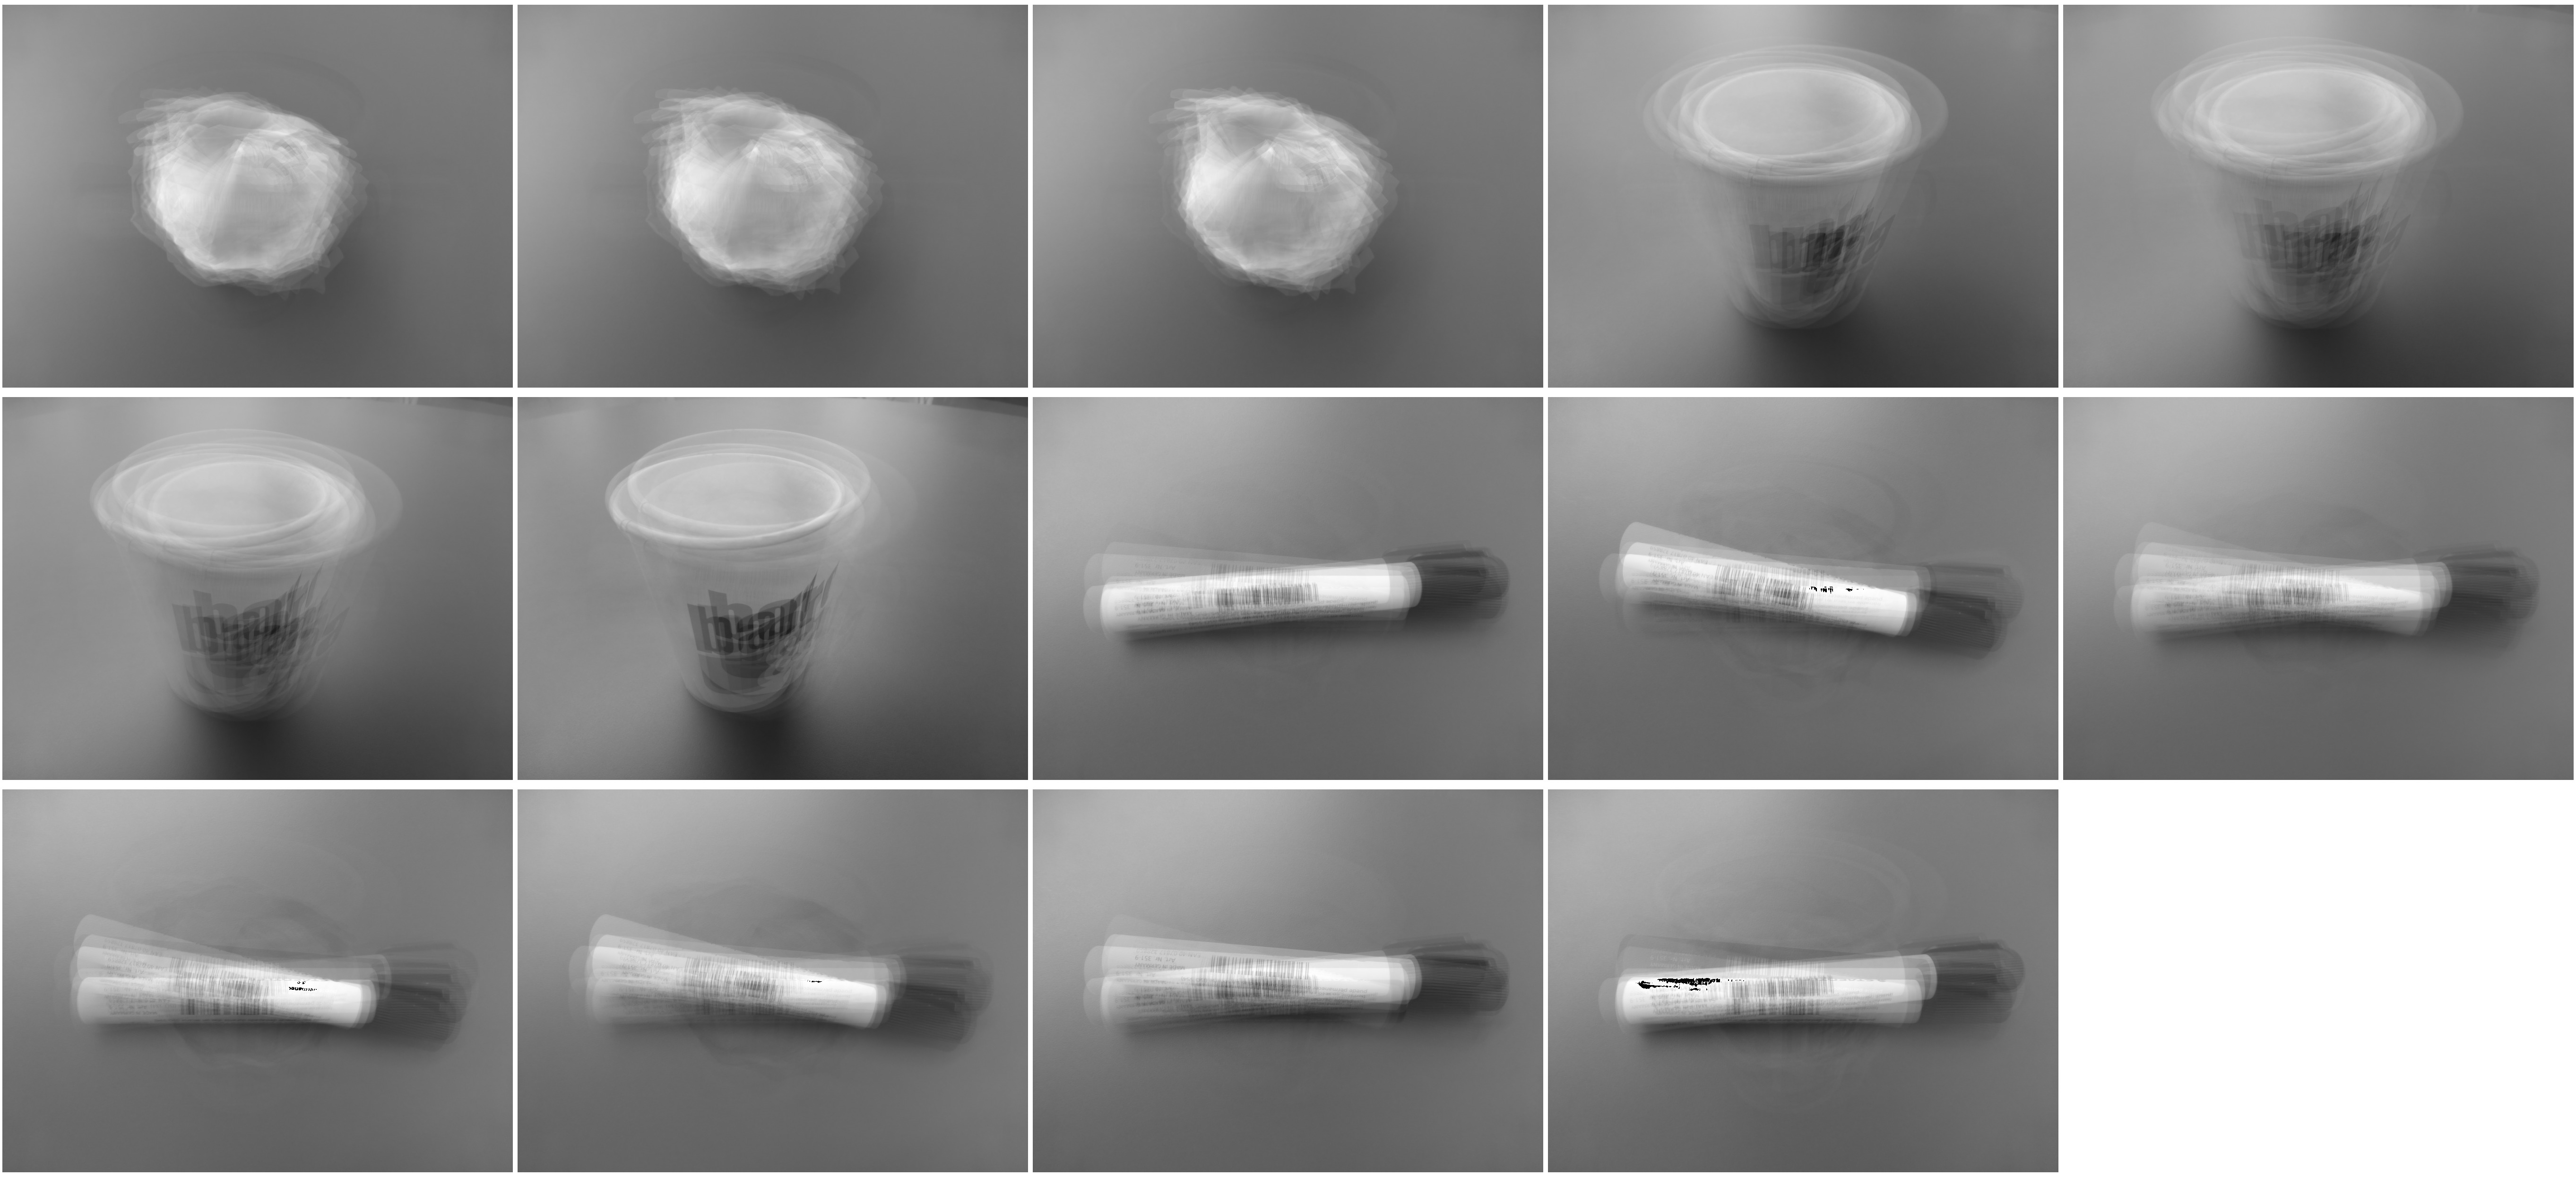
\includegraphics[height=7.5cm]{img/princ}
    \caption{Images representing inverse-tarnsformations of baycenter points of each of the principal simplices ordered by decreasing sizes of simplices.}
    \label{fig:princ_barycenters}
\end{figure}

\begin{paragraph}{Principal simplices}are simplicies which are not faces of any bigger complex. In the built VR-cx we observed 14 principal simplicies, which are drawn in figure~\ref{fig:vr_princ}. We can notice that each of the principal simplicies is connecting points within same classes. In~\ref{fig:princ_barycenters} the images representing barycenteer points of each of the principal simplices are presented. It is interesting to see that there are as many principal simplicies connecting ``pen''-points, as there are ``paper'' and ``cup'' principal simplicies all together. The intuition for this is that since pen is a ``pointy'' object, small rotations of the image cause bigger changes in the image than if the object is rounder (which is the case at paper and cup images).

  \todo{[A] Explain that simplices of larger dimension are just about useless}


\end{paragraph}

\begin{paragraph}{Intercluster edges}  
  \todo{[A] Pick one (or several) edges in V1 which is not in V2 and reconstruct the image corresponding
to the midpoint. This should somehow capture the difference between the
two components connected by this edge. Does it?}
\end{paragraph}

\end{homeworkSection}


\begin{homeworkSection}{General classification}

  \todo{[R] Explain we get same results as with S-L clustering, and with that the same problems as S-L clustering.}

  \todo{[R] Show bad results on our first dataset.}

  \todo{[A] Extra tests: iris, \ldots}

\begin{paragraph}{Modifying algorithm to prefer simplices of larger dimension.}  
  Because we proved that our basic model that only considers simplices of dimension 1 produces identical results as single-linkage clustering algorithm, and because VR cx can produce simplices of higher dimensions, we wondered if we could somehow use those to increase robustness of our algorithm. The main idea is that if some vertices are present in a simplex of higher dimension, they are more likely to be a part of the same class (since all the points are bunched up closer together). Unfortunately this turned out to be useless in practice, as even simplices of higher dimension are still built based on some distance metric between points, and if two clusters of different classes are close enough together, they may form a simplex of very large dimension resulting in a incorrect classification. The idea also would not work too well on thin, long clusters as seen in figure \ref{fig:mds_preprocessing}. On top of everything, this would also add a second parameter (dimension in addition to $r$), that the model has to balance out to produce desired number of clusters, and we would have to construct simplices of dimensions $\ge 1$ at each run of VR algorithm, further increasing the computational complexity with potentially no benefit.
\end{paragraph}

\end{homeworkSection}
\end{homeworkProblem}

\begin{homeworkProblem}[Summary]

  \todo{[A] Brief summary}

  \todo{[A] Further work (if there even is any), what we didn't explore.}
\end{homeworkProblem}

\begin{homeworkProblem}[Workload]

  \todo{Write here about your work on the project and I ([A]) will then summarize it into a paragraph or two.}
  \begin{itemize}
    \item P: Prepared Preprocessing class (StandardScaler, PCA), prepared VR-cx, added MDS visualizations, tested different scalers.
    \item R:
    \item A: Implemented methods for loading/saving images, preparing the dataset for use in the model, implemented the model, converted original images to grayscale and resized them,
  \end{itemize}
\end{homeworkProblem}
A more detailed overview of each member's workload can be seen at github repository of our project: \url{https://github.com/ptrus/vietoris_rips_image_classification/commits/master}.


\bibliography{./bib}{}
\bibliographystyle{plain}

\end{document}
